%bra paket
\documentclass[twocolumn]{article}
\usepackage[utf8]{inputenc}
%\usepackage[swedish]{babel}
\usepackage{fancyhdr}
%\usepackage{times}
%\usepackage{alltt} %verbatim text med möjlighet till andra latexkommandon i.
%\usepackage[usenames,dvipsnames]{color} %fler färger att välja på
%\usepackage{wrapfig} %figurer som ligger sida vid sida med texten
%\usepackage[table]{xcolor} %bakgrundsfärg i tabeller
%\usepackage[small,compact]{titlesec} %Spara plats!!
\usepackage{amsmath}
\usepackage{multicol}
\usepackage{graphicx}
\usepackage{float} %gör så att man kan placera bilder exakt mha [H]
\usepackage[table]{xcolor} %bakgrundsfärg i tabeller

%\usepackage[ddmmyyyy]{datetime}

\usepackage{setspace}
%\usepackage[usenames,dvipsnames]{color} %fler färger att välja på
%\usepackage{pdfpages} %för att kunna använda includepdf i appendix
\usepackage{pgf}
\usepackage{tikz}
\usetikzlibrary{arrows,automata}
\usetikzlibrary{positioning}
\tikzset{
    state/.style={
           rectangle,
           draw=black, thick,
           minimum height=3em,
           inner sep=5pt,
           text centered,
           },
}

% Different font in captions
\newcommand{\captionfonts}{\em}
\makeatletter  % Allow the use of @ in command names
\long\def\@makecaption#1#2{%
  \vskip\abovecaptionskip
  \sbox\@tempboxa{{\captionfonts #1: #2}}%
  \ifdim \wd\@tempboxa >\hsize
    {\captionfonts #1: #2\par}
  \else
    \hbox to\hsize{\hfil\box\@tempboxa\hfil}%
  \fi
  \vskip\belowcaptionskip}
\makeatother   % Cancel the effect of \makeatletter


%marginaler
\setlength\topmargin{0in}
\setlength\headheight{11pt}
\setlength\textheight{8.1in}
\setlength\textwidth{6.5in}
\setlength\oddsidemargin{0in}
\setlength\evensidemargin{0in}
\setlength\parindent{0in}
\setlength\parskip{0in}
\frenchspacing %Oui!

%För att kunna typsätta delar för sig!
\newcommand{\master}{}

%då kör vi


\begin{document}
%%%%%%%%%%%%%%%%%%% Försättsblad %%%%%%%%%%%%%%%%%%%%%%%%
\begin{titlepage}
\title{\textbf{Electric lab-assistant} \\
\Large{Engineering Applications using Matlab}\\
\large{TNG016}}
\author{
\vspace{30pt}\\
\large
ED3:\bigskip \\
\begin{tabular}{l l}
	Dan	Helgesson & danhe046 \\
	Albert Skog	& albsk635 \\
	Karl Westerberg	& karwe772 \\
\end{tabular}\vspace{40pt}\\
Examiner: Qingxiang Zhao 
}
\date{Submitted: \today}
\maketitle
\thispagestyle{empty}
\begin{center}


\begin{figure}[b]
	\begin{center}
		
\includegraphics[scale=0.6]{Figure/LIU-logo.jpg}
	\end{center}
\end{figure}

\end{center}

\end{titlepage}

%%%%%%%%%%%%%%%%%%% Header %%%%%%%%%%%%%%%%%%%%%%%
\pagestyle{fancy}
\fancyhead[l]{Engineering Applications using Matlab\\Electric Lab-Assistant}
\fancyhead[r]{Dan Helgesson, Albert Skog\\ \& Karl Westerberg}
\fancyfoot[c]{}
%%%%%%%%%%%%%%%%%%% Contents %%%%%%%%%%%%%%%%%%%%%
\onecolumn
\tableofcontents
\clearpage
\setcounter{page}{1}
\fancyfoot[c]{\thepage}
\twocolumn


%%%%%%%%%%%%%%%%%% Rapporten %%%%%%%%%%%%%%%%%%%%%
\section{Introduction}
%Om filen typsätts som del av hela rapporten så finns \master definierat i början och ingen \begin{document} och \end{document} får finnas, men för att kunna typsätta filen för sig är dem ett måste! \newcommand{\master}{} krävs i början på huvudrapporten!
\ifdefined\master
\else
	\documentclass[twocolumn]{article}
	\input{../preamble}
	\begin{document}
\fi
%text goes here!









\ifdefined\master
\else
	\end{document}
\fi

\section{Lab-Assistant}

The user interface of Lab-Assistant is designed to be intuitive and user-friendly. When launched the user is met by three empty columns, each with a popup-menu at the top. The columns are called \emph{input}, \emph{output} and \emph{export}, each with a set of 3-4 different options. Using different combinations of these options, a variety of tasks can be performed.
%Om filen typsätts som del av hela rapporten så finns \master definierat i början och ingen \begin{document} och \end{document} får finnas, men för att kunna typsätta filen för sig är dem ett måste! \newcommand{\master}{} krävs i början på huvudrapporten!
\ifdefined\master
\else
	\documentclass[twocolumn]{article}
	%\input{../preamble}
	\begin{document}
\fi
\subsection{Inputs}
Lab Assistant supports two types of devices for input; function generators and voltage generators. The function generator can also be used to generate a frequency sweep.
\subsubsection*{Function Generator}
Uses function generator to output a signal. The \emph{waveform} popup-menu sets the signal type to sine, square, triangle or sawtooth. If no waveform is selected the current waveform of the function generator is used. \emph{Frequency}, \emph{amplitude} and \emph{offset} controlls the parameters of the output. In order to establish a connection to the function generator its GPIB-address must be put into the \emph{GPIB-address} field.

\subsubsection*{Frequency Sweep}
The function generator can also be used to generate a Bode plot of a connected system. When \emph{frequency sweep} is selected as input, output is automatically set to \emph{bode graph} and no other outputs can be chosen. Available settings for the sweep are \emph{start frequency}, \emph{end frequency}, \emph{step length} and \emph{amplitude}. GPIB-address must allso be filled in as described above.

\subsubsection*{Voltage Generator}
The other device supported is the voltage generator. Apart from \emph{GPIB-Address} of the voltage generator, the available settings are \emph{voltage} and \emph{current limit}. Output can be toggled with the \emph{output on/off} pushbutton.


\ifdefined\master
\else
	\end{document}
\fi
%Om filen typsätts som del av hela rapporten så finns \master definierat i början och ingen \begin{document} och \end{document} får finnas, men för att kunna typsätta filen för sig är dem ett måste! \newcommand{\master}{} krävs i början på huvudrapporten!
\ifdefined\master
\else
	\documentclass[twocolumn]{article}
	\usepackage{graphicx}
	\usepackage{float}
	\usepackage{alltt}
	\begin{document}
\fi

\subsection{Outputs}
Two methods of gathering output data are available

\subsubsection*{Oscilloscope}
The oscilloscope has two functions, \emph{picture} and \emph{measurement} shown in Figure \ref{fig:osc}. The picture option practicaly takes a copy of the oscilloscope screen and shows it in the panel. The measurement option is used for getting the graph and plot with Matlab without all extra information the oscilloscope shows. The plot is then displayed in the panel. After entering the \emph{GPIB address} for the oscilloscope, the \emph{Start} button will execute the option chosen. (Figure \ref{fig:osc})

\begin{figure}[H]
\centering
\fbox{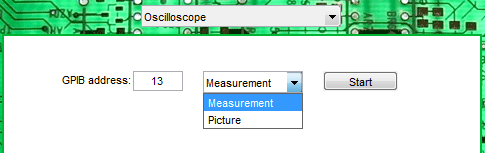
\includegraphics[width=6cm]{Figure/out_oscilloscope.png}}
\caption{Oscilloscope output settings.}
\label{fig:osc}
\end{figure}

\subsubsection*{Multimeter}
The multimeter function is just a multimeter, that displays the value in the panel as shown in Figure \ref{fig:multi}. When the \emph{Start} button is hit the multimeter begins uppdating the value in the panel. When the \emph{Stop} button is hit the multimeter stops updating and instead plot all previous values in a stem plot. (Figure \ref{fig:multi})

\begin{figure}[H]
\centering
\fbox{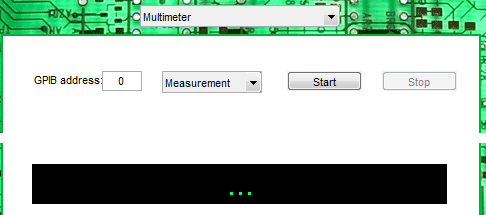
\includegraphics[width=7cm]{Figure/Multimeter.png}}
\caption{Multimeter output settings.}
\label{fig:multi}
\end{figure}

\subsubsection*{Bode Graph}
When the frequency sweep is chosen in the input panel it automaticaly chose the bode graph in the output panel. The Bode Graph only works with the frequency sweep as the start button is placed in the input panel. The plot is shown in the output panel. (Figure \ref{fig:bode})

\begin{figure}[H]
\centering
\fbox{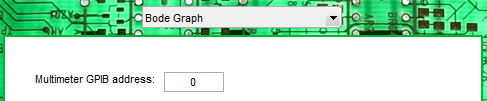
\includegraphics[width=6cm]{Figure/bode_graph.png}}
\caption{Bode plot output settings.}
\label{fig:bode}
\end{figure}


\ifdefined\master
\else
	\end{document}
\fi
%Om filen typsätts som del av hela rapporten så finns \master definierat i början och ingen \begin{document} och \end{document} får finnas, men för att kunna typsätta filen för sig är dem ett måste! \newcommand{\master}{} krävs i början på huvudrapporten!
\ifdefined\master
\else
	\documentclass[twocolumn]{article}
	%\input{preamble}
	\begin{document}
\fi
\subsection{Exports}
The program has four different choices for exporting the obtained data; copy to clipboard, save as image, create LaTeX report and create Microsoft Word report.

\subsection*{Clipboard}
Copies the figure to clipboard. Textboxes enable the user to modify title and axis labels before copying.

\subsection*{Image}
Saves the image to disk. Textboxes enable the user to modify title and axis labels before copying.

\subsection*{LaTeX}
Generates LaTeX report containing the figure. \emph{Image name} textbox enables user to choose file name and format for the figure, which will be saved at the same location as the tex-file. \emph{Caption}, \emph{label} and \emph{width} properties are transferred to corresponding LaTeX commands, while tite and labels are applied directly to the figure before exporting. 

\subsection*{Word}
Generates Microsoft Word report containing the figure. \emph{Title}, \emph{x-label} and \emph{y-label} overrides the settings of the figure and the caption is inserted on a centred line below.




\ifdefined\master
\else
	\end{document}
\fi

%Om filen typsätts som del av hela rapporten så finns \master definierat i början och ingen \begin{document} och \end{document} får finnas, men för att kunna typsätta filen för sig är dem ett måste! \newcommand{\master}{} krävs i början på huvudrapporten!

\ifdefined\master
\else
	\documentclass[twocolumn]{article}
\usepackage{graphicx}
\usepackage{float} %gör så att man kan placera bilder exakt mha [H]
	%\input{../preamble}
	\begin{document}
\fi
%text goes here!
\section{Lab demonstration}
To demonstrate the functionality of the program an easy lab-assignment is performed. A RC-circuit was connected like figure \ref{fig:RCcircuit}, the circuit is a low-pass filter with the cutoff frequency at $f=1.5~kHz$. 
	\begin{figure}[h]
	\centering
		\fbox{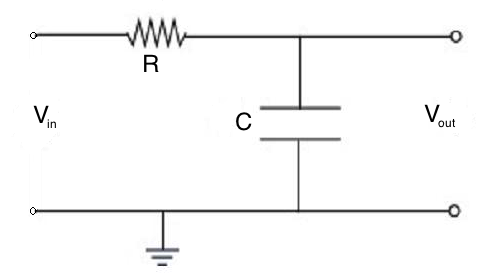
\includegraphics[width=5cm]{Figure/rc-circuit}}
		\caption{RC-circuit}
		\label{RCcircuit}
	\end{figure}

Start with connecting the oscilloskop, multimeter, function- and voltage generator to the computer using the GIPB-port, you need to check that every device have a different GPIB-address to be sure that all will work.  

\subsection{Assignment 1}
The first assignment is about looking at the difference between the in- and out-signal. Set the function generator to a frequency at $1~kHz$ and the amplitude to $3~V$ you also need to add the GIPB-address of the function generator and the oscilloskop. Click at \emph{Set} bottom in the function generator panel and select \emph{oscilloskop picture} in the popup-menu at the out panel an then. Now you need to add the GPIB-address to the oscilloskop and click start to get a picture from the oscilloskop. Figure \ref{oscilloskopPicture} shows a picture from the oscilloskop whit the settings mentioned above. 
	\begin{figure}[h]
	\centering
		\fbox{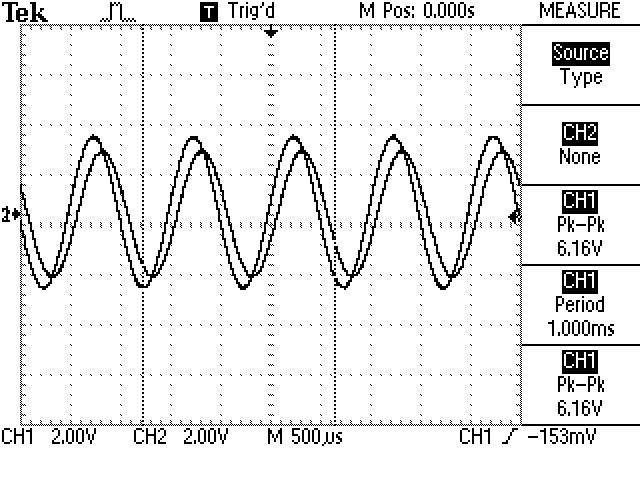
\includegraphics[width=6cm]{Figure/screenshot.png}}
		\caption{Oscilloscope picture.}
		\label{oscilloskopPicture}
	\end{figure}

Now we wont to use the export function to implement the figure in a report. By selecting the \emph{LaTeX} alternate in export popup-menu, your able to change the title and  figure labels  by typing the wonted label name in the \emph{X-Label} and \emph{Y-Label} text boxes, the figure title is chanced by typing in the \emph{Title} text box. You can also set the LaTeX figure caption and reference label by typing in the \emph{Label} and \emph{Caption} text boxes. Than it's jest to type a figure name and click \emph{export} and chose a location for the file to be saved.

\subsection{Assignment 2}
Connect the multimeter to measuring the voltage over the resistor. Change the output bar to multimeter, select the \emph{Voltage [AC]} in the measuring popup-menu, add the GPIB-address for the multimeter and press start button. Now you will see the multimeter display in the black text box in the out-panel. By clicking the \emph{Stop}-button you stop the multimeter and you can save the data in a .mat file and also present the measerment in a stem-graph by saving the figure. The generated stem-graph is presented in figure \ref{stem} 
	\begin{figure}[h]
	\centering
		\fbox{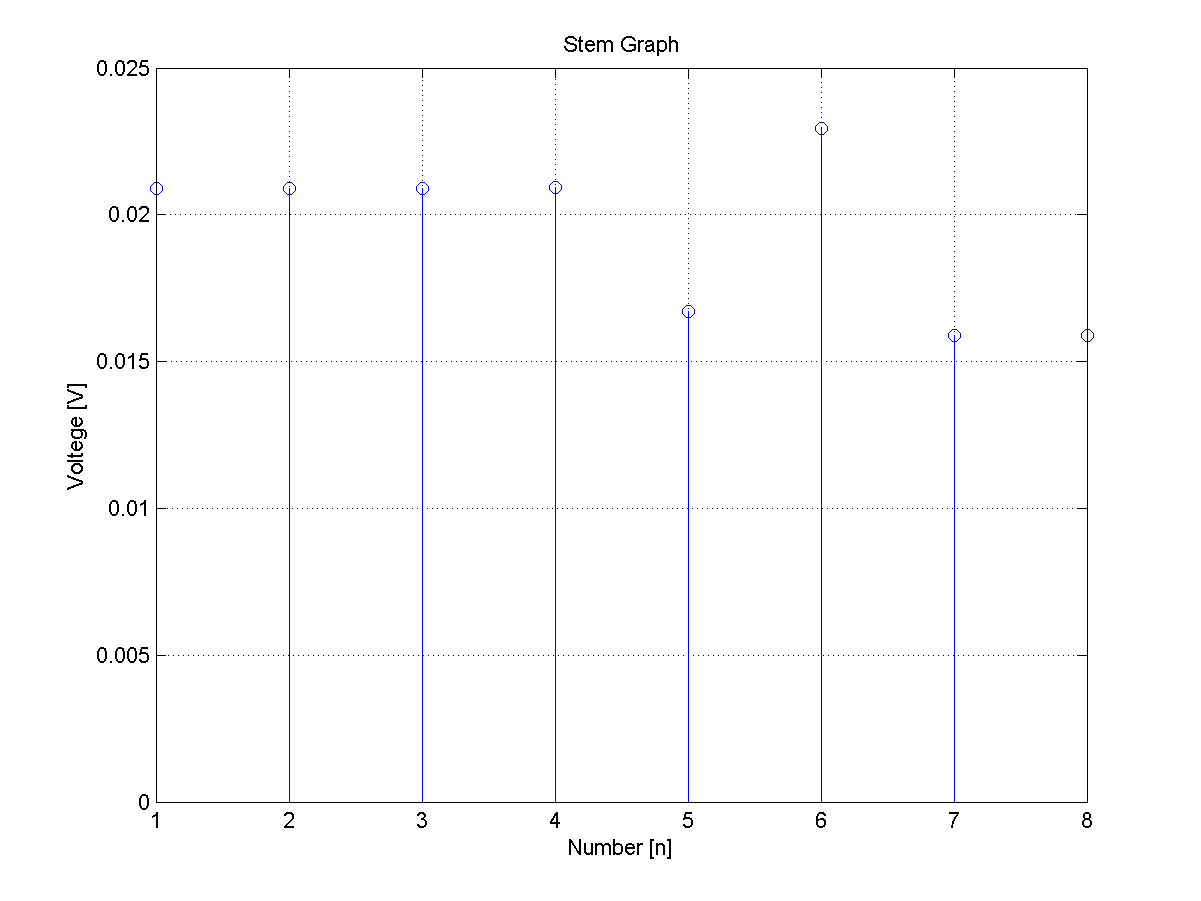
\includegraphics[width=6cm]{Figure/stem.png}}
		\caption{stem graph}
		\label{stem}
	\end{figure}

\subsection{Assignment 3}
Now move the multimeter probes to measuring the out voltage and change to \emph{frequency sweep} in the input popup-menu and set the start, end frequency to $0~Hz$ and $3000~Hz$ and the step length to $100~Hz$ use \emph{Sine} as waveform with an amplitude at $3~V$ and click \emph{Start sweep}. This will take some time.\\
\\
The generated bode graph figure \ref{bode} can be exported to a Word-document in the same way as the LaTeX export, the generated frequency and voltage can also be saved for other use in MATLABs workspace. 
	\begin{figure}[h]
	\centering
		\fbox{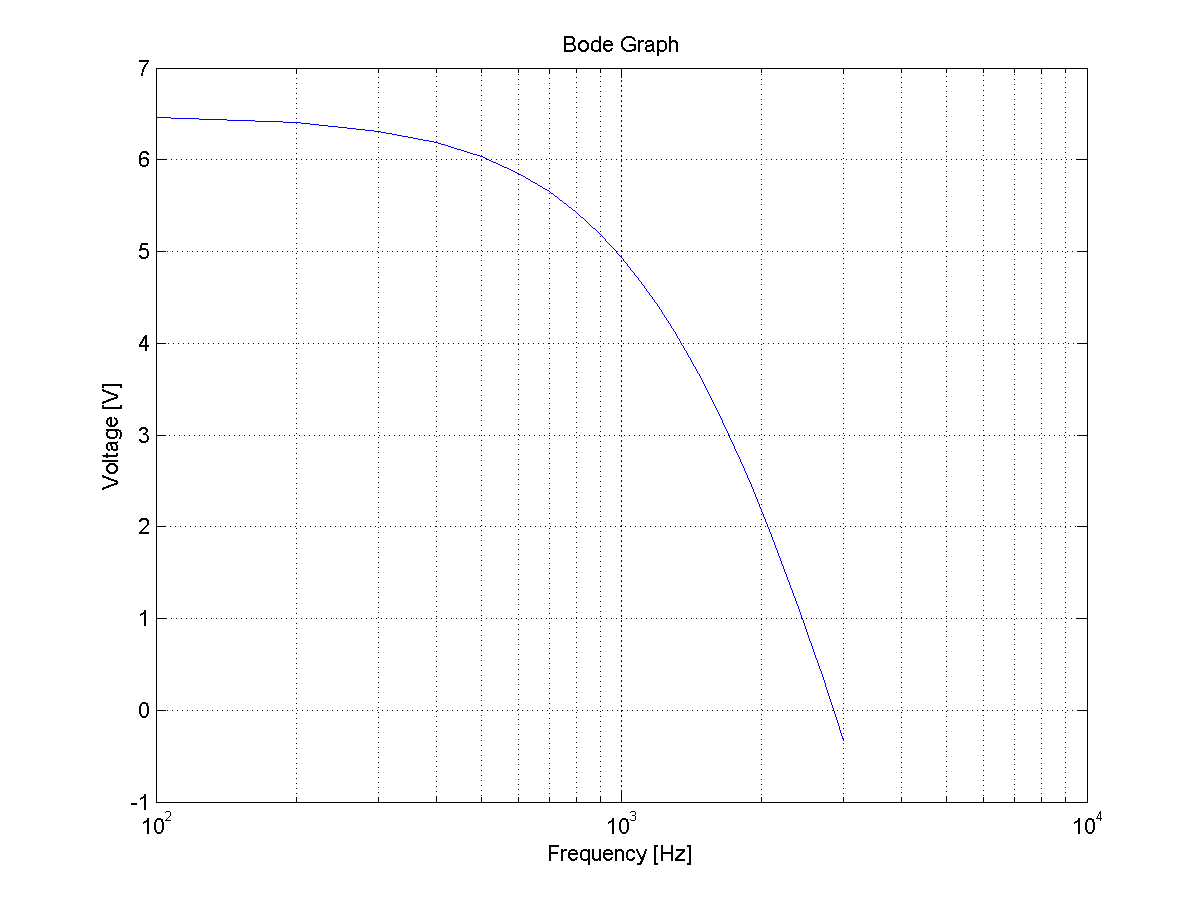
\includegraphics[width=6cm]{Figure/bode.png}}
		\caption{Bode graph}
		\label{bode}
	\end{figure}   

\ifdefined\master
\else
	\end{document}
\fi

\section{Conclusion}
%Om filen typsätts som del av hela rapporten så finns \master definierat i början och ingen \begin{document} och \end{document} får finnas, men för att kunna typsätta filen för sig är dem ett måste! \newcommand{\master}{} krävs i början på huvudrapporten!
\ifdefined\master
\else
	\documentclass[twocolumn]{article}
	\begin{document}
\fi


The Lab-Assistant is easy to use, but it would be possible to make it even more user friendly by making more intelligent dialogues for connecting the GPIB-devices, enabling models from other vendors etcetera. Overall, more of the device functionalities can be brought into the software, focus during the project has been diversity rather than depth on this part.\\

The program can always be improved with more functions and calculations. For example Matlab offers a lot of ways to modify colors, line types and other features of the obtained figure. Another way to go is adding different types of input methods beside GPIB, like serial or USB.\\

An interesting issue is the matter of special cases, such as the Bode plot generator, where one choice of the input reduces the number of available outputs to just one. How should this be solved in the user interface? Should the function generator pane have multiple modes, or should each mode have a different name in the input selection menu? The latter was chosen to highlight the dilemma and show a way to solve it; when the user chooses to perform a frequency sweep, Bode plot becomes the only output option available (for the sake of this argument, of course functionality could be developed for other output modes as well).\\
%inte riktigt kanske men det låter ju bra =)


It is indeed possible, as proven by the Lab-Assistant software, to make lab work more efficient by utilizing the power of Matlab to create a common user interface for commonly used equipment. Connecting control over multiple instruments with direct export of the results can definitely be done effectively on a PC.


\ifdefined\master
\else
	\end{document}
\fi

\end{document}